\documentclass{beamer}
 
\usepackage[utf8]{inputenc}
\usepackage{graphicx}
 
 
%Information to be included in the title page:
\title{Aviones, delays, cuadrados mínimos...\\ y un poco del viejo de la bolsa}
\author[]{Alfredo Umfurer \and Franco Assenza \and Kevin Maldonado}
\institute{Universidad de Buenos Aires}
\date{2019}
 

\begin{document}

\frame{\titlepage}

\begin{frame}
\frametitle{Table of Contents}
\tableofcontents
\end{frame}
  
\section{Objetivos del trabajo}\label{sec:objetivos-del-trabajo}
\begin{frame}
\frametitle{Objetivos del trabajo}
\begin{itemize}
\item El objetivo principal del trabajo es entender y poder predecir qué causa los delays de los vuelos de las aerolineas comerciales.\\
\begin{itemize}
\item<1-> Es culpa de las aerolineas?
\item<2-> Es culpa de la aleatoriedad del clima?
\item<3-> Es culpa de los aeropuertos sobrepasando su capacidad?
\end{itemize}
\item<4-> Además de esto, vamos a hacer un breve análisis para intentar entender los movimientos en bolsa de las aerolineas.
\end{itemize}
\end{frame}
 
\section{Marco Teórico}\label{sec:marco-teórico}
\begin{frame}
\frametitle{Marco Teórico}

Ideas:
\begin{itemize}
	\item<1-> Analizar distintos componentes responsables
	\begin{itemize}
		\item<2-> ajustar distintas funciones a los datos
		\item<3-> \textbf{Cuadrados mínimos} con la familia de funciones $\sum a_i \cdot \phi_i(x_i)$ donde las $\phi$ contemplan
		\begin{itemize}	
			\item<4-> Una componente lineal, que aparece con el crecimiento natural en el tránsito aéreo.
			\item<5-> Componentes periódicas sinusoidales, para capturar períodos temporales como temporadas, días de semana y horarios pico
			\item<6-> Una componente especialmente puntiaguda, para capturar los días festivos de fin de año.
			\item<7-> Componentes basadas en scores, de la aerolínea y de los aeropuertos
		\end{itemize}
	\end{itemize}
\end{itemize}
\end{frame}
\begin{frame}
\begin{itemize}
	\item<1-> Componentes impredecibles
	\begin{itemize}
		\item<1-> Clima
		\item<1-> Eventualidades relacionadas con los aeropuertos y las aerolíneas
		\item<1-> Eventos mundialmente relevantes
		\begin{itemize}
			\item<2-> Caidas de la bolsa
			\item<2-> 9/11
		\end{itemize}
	\end{itemize}
	\item<3-> Componentes fuera de nuestro alcance
	\begin{itemize}
		\item<3-> Bancarrotas de aerolíneas
		\item<3-> Fusiones de aerolíneas
	\end{itemize}
\end{itemize}

\end{frame}


%\begin{frame}
%\begin{itemize}
%	\item Mirar la bolsa la bolsa la bolsa
%\end{itemize}
%\end{frame}

\section{Metodología y datos}
\begin{frame}
\frametitle{Metodología y datos}
Los datos utilizados para el análisis son los de vuelos de aerolíneas comerciales estadounidenses en el período abarcado entre el 2003 y el 2008.
\begin{itemize}
\item Intencionalmente evitamos la crisis del 9/11 (2001) y la recesión del 2008.
\end{itemize}
Usamos la siguiente metodología para analizar los datos y sacar conclusiones
\end{frame}


\begin{frame}
\frametitle{Metodología y datos -  Linear Trending}
\\ Consiste en remover la componente lineal a los datos
  \centering
  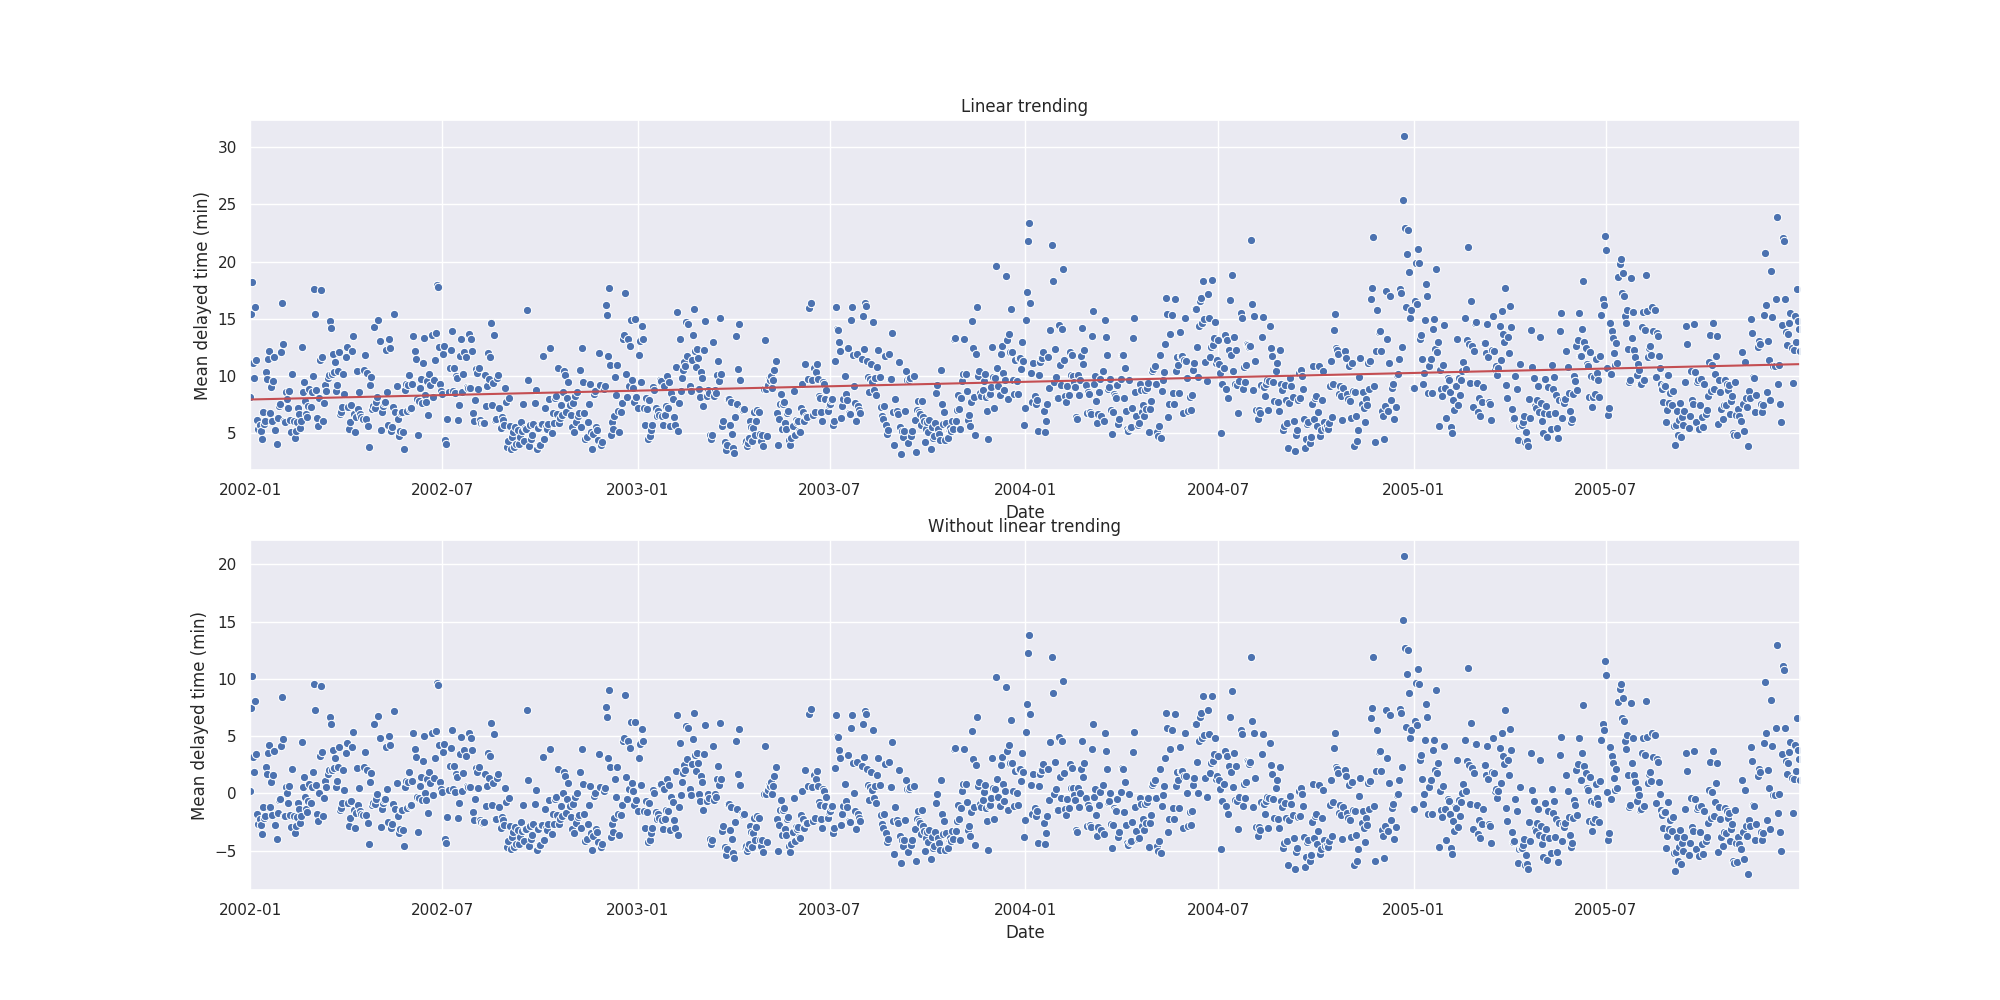
\includegraphics[width=0.8\textwidth]{plots/linear_trending.png}
\end{frame}


\begin{frame}
\frametitle{Metodología y datos - Funciones sinusoidales}
	\begin{itemize}
		\item<1-> Podemos ajustar usando una combinaci\'on lineal de senos y cosenos
		\item<2-> $c \times \sin(x + \alpha) = c \times \cos \alpha \sin x + c \times \sin \alpha \cos x$
		\item<3-> Solo necesitamos definir la amplitud.
		\begin{itemize}
			\item<4-> Asumiendo un comportamiento peri\'odico anual, elegimos frecuencias multplo de 365
		\end{itemize}
	\end{itemize}
\end{frame}

\begin{frame}
	\frametitle{Metodología y datos - D\'ia de la semana}

	\textbf{Idea:} Podemos usar el mismo enfoque que para el a\~no: tomar frecuencias semanales\\
	\pause
	\textbf{Otra idea:} Usar una funci\'on indicadora que evalue en 1 para una d\'ia y 0 en los dem\'as \\
	\pause
	\begin{itemize}
		\item \textbf{senos y cosenos:}, tenemos dos features por cada frecuencia
		\item \textbf{Indicadora:} Tenemos 7 features, uno por cada dia de la semana
	\end{itemize}


\end{frame}



\section{Descubrimientos}\label{sec:descubrimientos}
\begin	{frame}
\frametitle{Descubrimientos}
\begin{itemize}
\item No hay que volar con United porque te sacan del vuelo con un taser porque overbookean los vuelos
\end{itemize}

\end{frame}

\section{Trabajo Futuro}
\begin{frame}
\frametitle{Trabajo Futuro}
\begin{itemize}
\item Contemplar merges de aerolineas
\item Dónde podríamos construir un aeropuerto para mejorar los delays?
\item Qué aeropuerto es el más importante alivianador de delays?
\item Qué aeropuerto es el más importante para mantener a la red conectada?
\item Qué dato útil e interesante podemos sacar del dataset
\end{itemize}
\end{frame}

\end{document}
